\documentclass[a4paper,11pt]{article}
\usepackage[left=2.5cm, right=2.5cm, top=1.5cm, bottom=1.5cm]{geometry}
\usepackage{graphicx}
\usepackage{amssymb}
\usepackage{amsmath}
\usepackage{xcolor}
\usepackage[active,tightpage]{preview}
\usepackage{hyperref}
\usepackage{pythonhighlight}

\hypersetup{ %color attributes of citation, link, etc.
    colorlinks=true,
    linkcolor=blue,
    filecolor=gray,
    urlcolor=blue,
    citecolor=blue,
}

\setlength{\parindent}{0pt}

\renewcommand{\PreviewBorder}{1in}
\newcommand{\Newpage}{\end{preview}\begin{preview}}
\newcommand{\matlab}{\textsc{Matlab}} %very important and totally necessary addition
\newcommand{\parallelsum}{\mathbin{\!/\mkern-5mu/\!}}

\newcommand\Item[1][]{%
  \ifx\relax#1\relax  \item \else \item[#1] \fi
  \abovedisplayskip=0pt\abovedisplayshortskip=0pt~\vspace*{-\baselineskip}}

%'codify' text for snippets
\usepackage{xcolor}
\definecolor{codegray}{gray}{1}
\newcommand{\code}[1]{\colorbox{codegray}{\texttt{#1}}}


\graphicspath{ {../images/} }
           
\begin{document}
\begin{preview}
\title{\LARGE{\textbf{ECEN405 Lab 6 Report\\PI Controlled Buck Converter}}}
\author{Niels Clayton : 300437590}
\date{}
\maketitle
\hrule

\section*{Deliverables}

\begin{enumerate}
    \item \textbf{Buck Converter Bode Plot} \\

    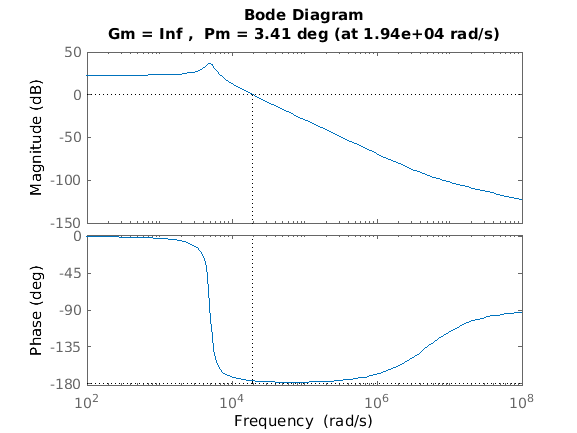
\includegraphics[width = \textwidth]{uncontrolled_buck.png}
    
    \begin{center}
        \textbf{\textit{Figure 1:}} Buck converter Bode plot with gain and phase margin displayed\\
    \end{center}


    \hrule
    \item \textbf{Controller Design} \\
    
    We are looking to design a PI controller, where the unity gain frequency (Phase Margin) of the original buck converter is unaffected. The following values were specified for the design:
    \begin{itemize}
        \item $R_i = 10k\Omega$
        \item $K_p$ = 0.1
    \end{itemize}

    From this the value of $R_f$ can be calculated using the following equation:

    \begin{align*}
        R_f &= K_p \cdot R_i\\
            &= 0.1 \cdot 10k\Omega\\ 
            &= 1k\Omega\\
    \end{align*}

    To ensure that the phase margin of the original buck is unaffected, we want the controller to have a phase of 0$^o$ at this location. From the transfer function of a PI controller it can be observed that it places a single zero on the S plain. This will cause a 90$^o$ phase shift from -90$^o$ over one decade, around the location of the integrating zero. By placing this integrating zero two decades below the phase margin of the original system we can guarantee that the phase of the controller will reach zero by this point. 

    Using this information, we can use the following equation to calculate the capacitor value required to place the zero two decades below the systems phase margin:

    \begin{align*}
        s &= -\frac{1}{R_f \cdot C}\\
        & \therefore\\
        C &= -\frac{1}{R_f \cdot s}\\
          &= -\frac{1}{1000 \cdot 1.94\cdot10^4}\\
          &= -5.17 \cdot 10^{-6}\\\\
          &= 5.17u\mathrm{F}
    \end{align*}

    The final component values are:
    \begin{itemize}
        \item $R_i = 10k\Omega$
        \item $R_f = 1k\Omega$
        \item $C = 5.17uF$\\
    \end{itemize} 

    \hrule
    \item \textbf{Controller Bode Plot} \\

    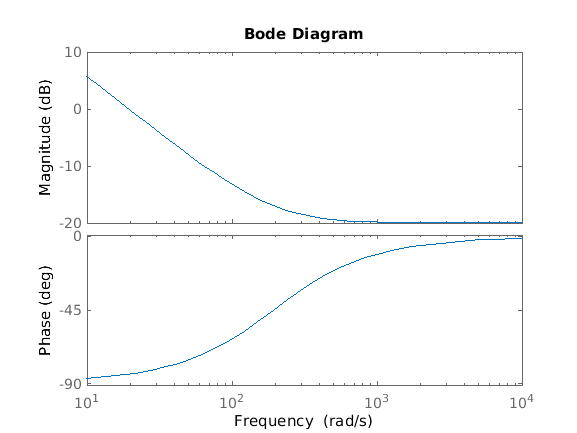
\includegraphics[width = \textwidth]{controller.png}
    
    \begin{center}
        \textbf{\textit{Figure 2:}} Controller Bode plot\\
    \end{center}


    \hrule
    \item \textbf{Controlled Buck Converter Bode Plot} \\

    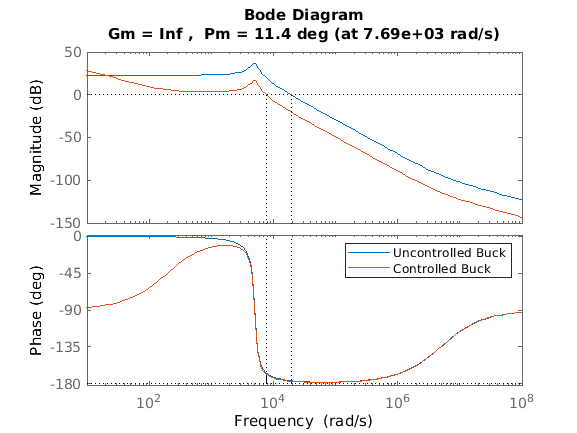
\includegraphics[width = \textwidth]{controlled_buck.png}
    
    \begin{center}
        \textbf{\textit{Figure 3:}} Controlled Buck converter Bode plot with the new gain and phase margin displayed\\
    \end{center}


    \hrule
    \item \textbf{Controlled Buck Converter Simulation} \\

    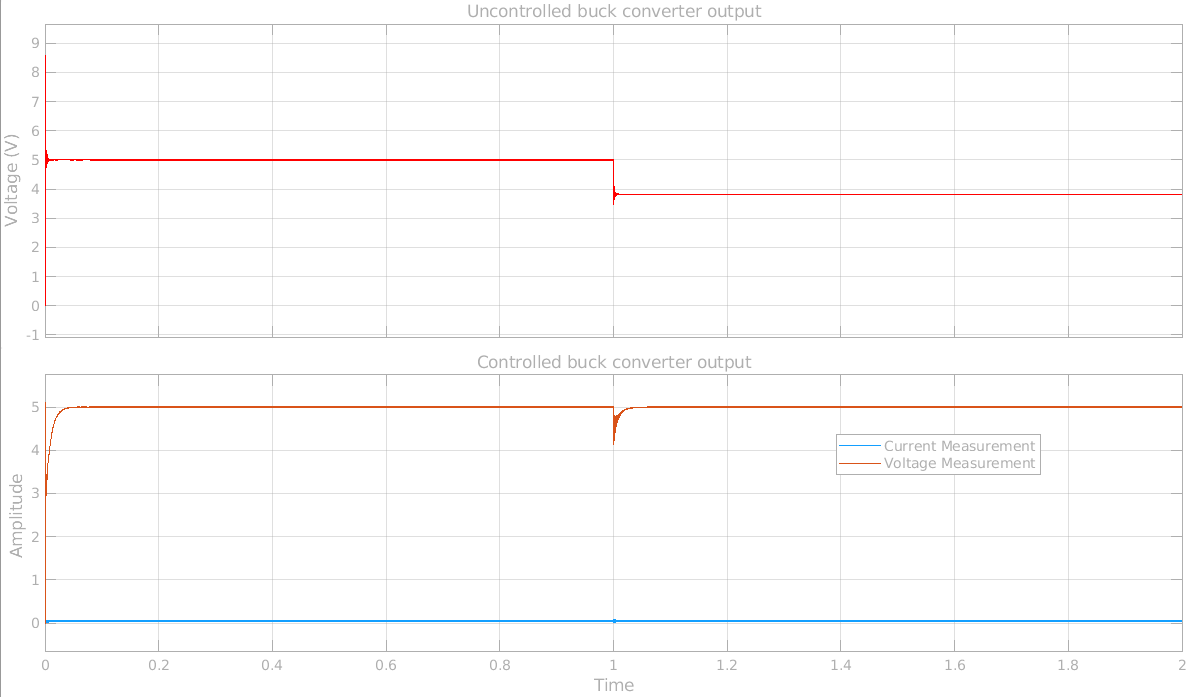
\includegraphics[width = \textwidth]{pi_sim.png}
    
    \begin{center}
        \textbf{\textit{Figure 4:}} Controlled buck converter vs uncontrolled buck converter simulation\\
    \end{center}


    \hrule
    \item \textbf{Controlled Buck Converter Implementation Schematic} \\

    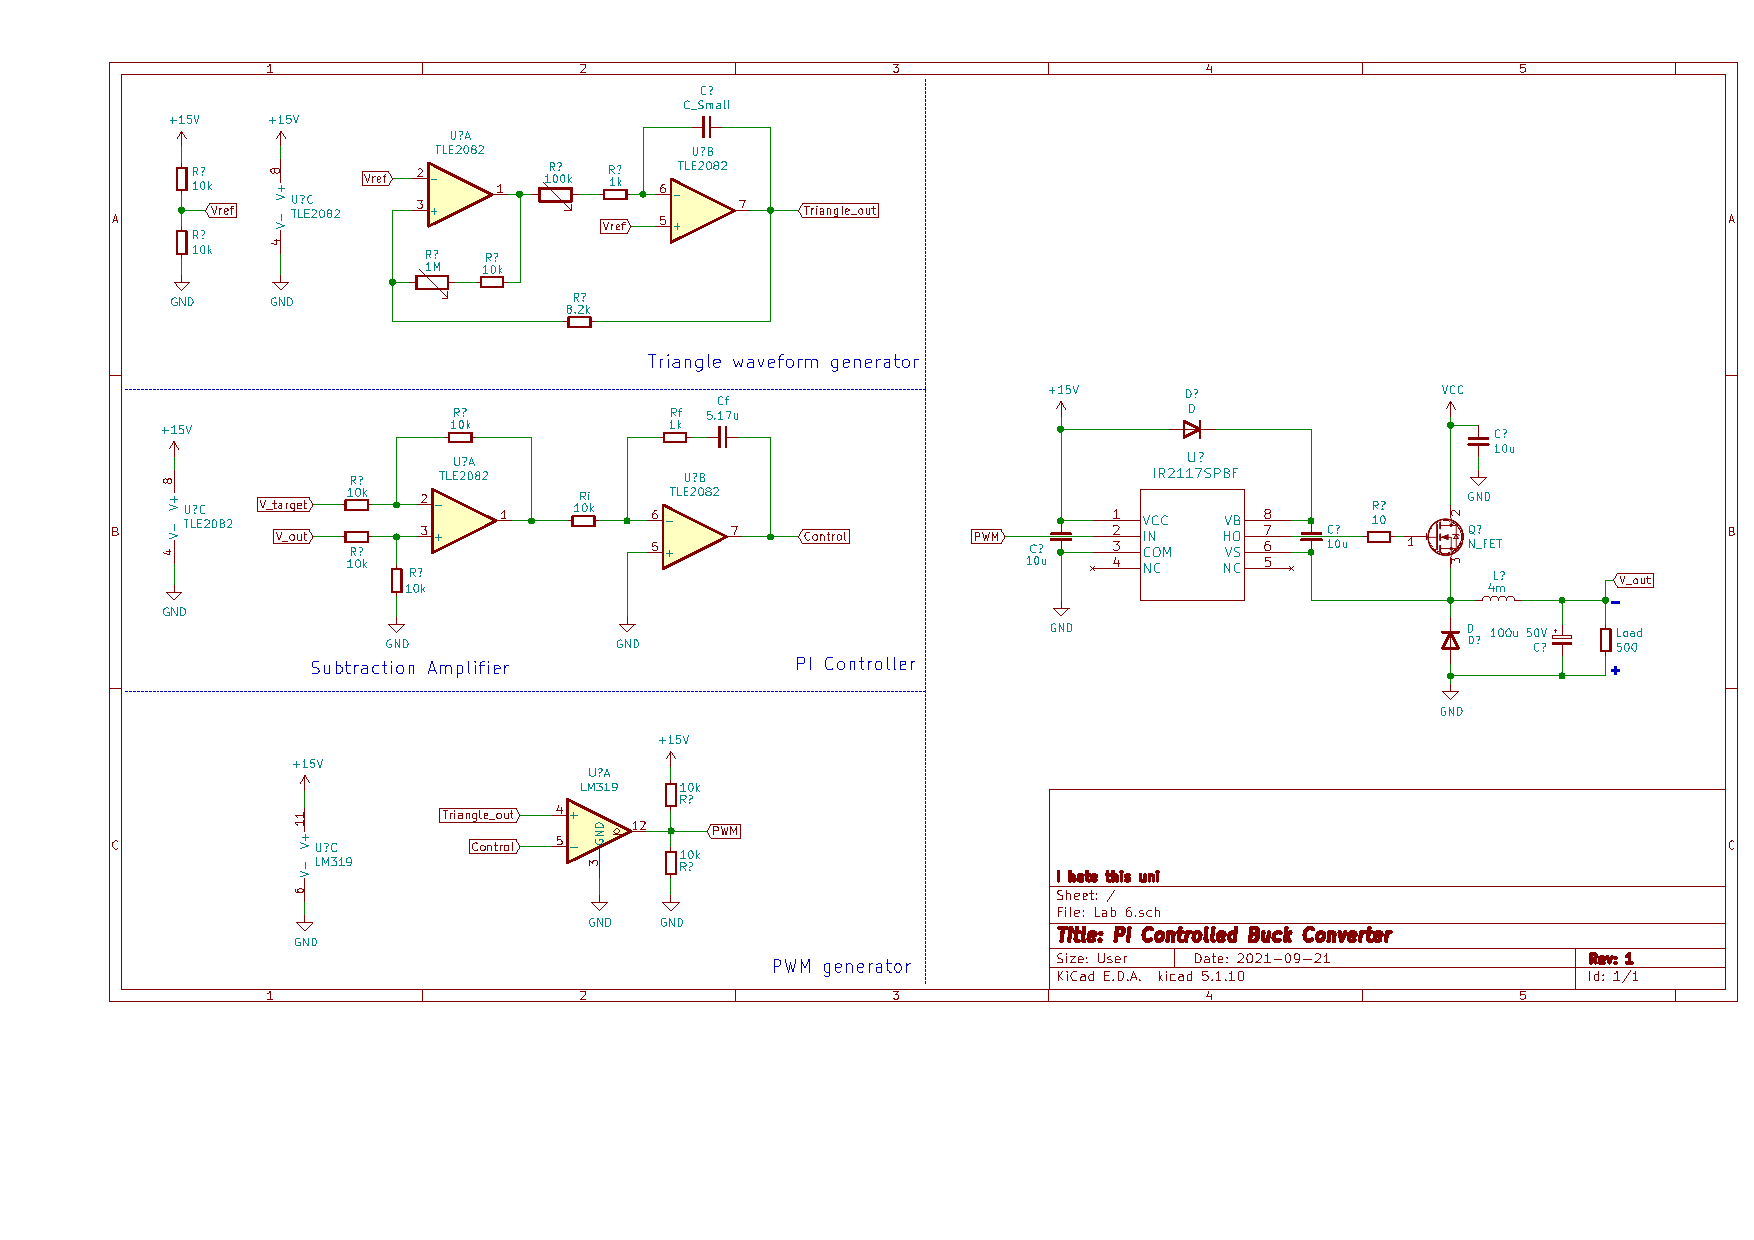
\includegraphics[width = \textwidth]{shem.pdf}
    
    \begin{center}
        \textbf{\textit{Figure 5:}} Controlled Buck Converter Implementation Schematic with relevant IC pinouts
    \end{center}



\end{enumerate}

\end{preview}
\end{document}